% Chapter 2

\chapter{Motivación} % Chapter title
\label{ch:motivacion}
\lhead{\emph{Motivación}}
%----------------------------------------------------------------------------------------
Hay numerosas motivaciones para la investigación de un nuevo método de 
calibración:
    
Primero, a la hora de adquirir imágenes satelitales es crucial que se 
conozca perfectamente la señal emitida y recibida por la antena. Ya sea por 
envejecimiento de los materiales, por variaciones de temperaturas u algún 
otro factor, se observan dispersiones de las mismas. Hay dos enfoques para 
encarar esta problemática:

\begin{itemize}
    \item Controlando las dispersiones máximas que pueden presentarse 
    utilizando hardware más complejo.

    \item Corrigiendo dichas dispersiones haciendo uso de calibración 
    interna.
\end{itemize}

Al utilizar la calibración interna se evita aumentar la complejidad y 
peso del hardware utilizado a costa de un mayor procesamiento de software, 
logrando así, disminuir el costo de la misión.
    
Otro motivo es que el método de calibración convencional posee numerosas
limitaciones y falencias; la principal es que no abarca todo el sistema de 
transmisión/recepción, dejando así parámetros fuera de control. 




\begin{comment}
El descubrimiento de la celda de combustible derivó de un experimento de electrólisis, proceso en el que se utiliza corriente
eléctrica para producir la separación de los compuestos en sus elementos. El hecho que llevó a descubrir el principio de la celda
de combustible fue la reversibilidad (en términos cualitativos) del proceso, es decir que pudo obtenerse energía eléctrica de
la reacción que devolviera los elementos al compuesto original.

La reacción química llevada a cabo es la misma que si el proceso fuese realizado mediante la combustión de los reactivos. 
Pero se distingue de éste último proceso en que parte de la energía liberada es eléctrica.
Por otra parte, la reversibilidad del proceso le confiere características particulares. Una de ellas
es que su eficiencia no está limitada por el ciclo de Carnot, como es el caso de los procesos termodinámicos.

\section{Principios de funcionamiento}

El dispositivo esta constituido básicamente por dos partes fundamentales: el electrolito y los electrodos. El electrolito es
el material que facilita el movimiento de iones y los electrodos ofrecen una superficie para la posibilitar la reacción química.
La reacción producida por las celdas más elementales y las de interés para este trabajo es la siguiente:

$$
2H_{2}+O_{2} \rightarrow 2H_{2}O
$$

Ésta última expresión sirve para ilustrar la simplicidad de los procesos químicos que se llevan a cabo en estos dispositivos.
El esquema de una celda de combustible elemental de electrolito ácido se muestra en la fig. \ref{fig:esquema_celda} con las
reacciones que entran en juego y el modo en que se da el flujo de los reactivos y productos entregando corriente eléctrica
a la carga conectada.

\begin{figure}[H]
 \centering
 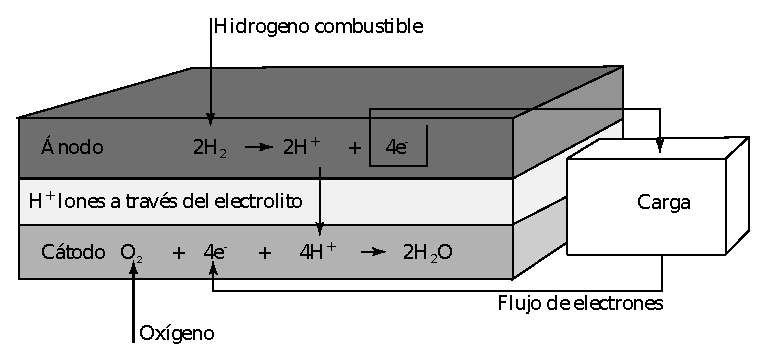
\includegraphics[width=10cm]{gfx/esquema_celda.eps}
 \caption{Esquema constructivo de una celda de combustible de electrolito ácido}
 \label{fig:esquema_celda}
\end{figure}

En el esquema de la fig. \ref{fig:esquema_celda} se analiza con mayor detalle las reacciones puestas en juego que se transcriben
en las ecuaciones \ref{eq:reacciones}.

\begin{subequations}
 \begin{equation}
  2H_2 \rightarrow 4H^{+}+4e^{-}
  \label{eq:reaccion_hidrogeno}
 \end{equation}
 \begin{equation}
  O_2+4H^{+}+e^{-} \rightarrow H_{2}O
 \end{equation}
 \begin{equation}
  2H_2+O_2 \rightarrow H_{2}O+ \Delta \overline{g}_f
  \label{eq:reaccion_basica}
 \end{equation}
 \label{eq:reacciones}
\end{subequations}

En ( \ref{eq:reaccion_basica}) se ha adicionado el término $\Delta \overline{g}_f$ que representa la energía de formación. 
Éste término es negativo para la reacción en cuestión, es decir que se libera energía de la reacción estudiada. Ésta energía
se manifiesta de diferentes maneras.

A pesar de tratarse de una reacción espontánea no se lleva a cabo a menos que se suministre la energía de activación necesaria
para que se produzca, y esto limita su ritmo. Para que aumente la probabilidad de que la reacción tenga lugar pueden
tomarse medidas como:
\begin{itemize}
 \item El aumento del área efectiva de los electrodos
 \item El aumento de la temperatura
 \item El uso de catalizadores
\end{itemize}

Si bien las celdas de combustible efectivamente proveen energía eléctrica, lo hacen en pequeñas cantidades. La tensión entregada entre
los terminales de sus electrodos es del orden de $1V$ y es por ello que normalmente las celdas de combustible se suelen configurar en
arreglos de \emph{pilas de celdas de combustible}, cuyas celdas son interconectadas en serie para que de los electrodos terminales 
se obtenga la suma de la tensión que entrega cada una de ellas.

Considerando la reducida tensión que entregan las celdas se disponen en pilas usando conectores especiales que limitan la caída de tensión
entre los contactos de cada electrodo. Una de las disposiciones típicas de las pilas de celdas es la que se muestra en la fig. \ref{fig:apilado}.

\begin{figure}[H]
 \centering
 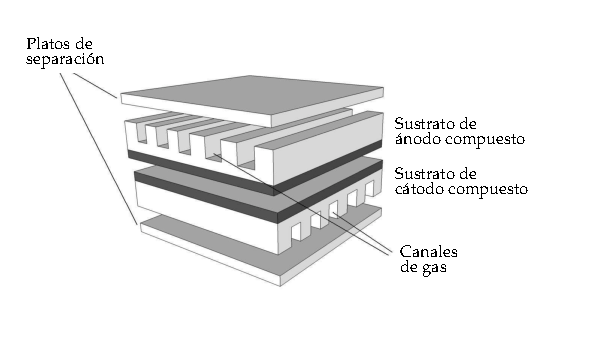
\includegraphics{gfx/apilado_bipolar_planar.eps}
 \caption{Disposición en apilado bipolar planar}
 \label{fig:apilado}
\end{figure}

\section{Tipos de celdas de combustible}
Para hacer frente a las dificultades presentadas en el desarrollo de las celdas de combustible, se probaron varias tecnologías dando
lugar a varios tipos de celdas de combustible. Éstas se diferencian especialmente por el electrolito utilizado y por ende el tipo
de ion que se mueve a través de él. En el cuadro \ref{tab:tipos_de_celdas} se listan las celdas típicas que pueden encontrarse.

\begin{table}[H]
 \centering
 \rowcolors{1}{}{gray!20}
 \begin{tabular}{|p{4cm}|p{1cm}|p{3cm}|p{5cm}|} \hline
 \rowcolor{LightBlue2} Tipo de celda de combustible	& Ion móvil	&Temperatura de operación	&Aplicaciones \\ \hline
 Alcalina (AFC)						& $ OH^{-} $	&$50-200$\textcelsius		&Usada en vehículos espaciales \\
 Membrana de intercambio de protones (PEMFC)		& $ H^{+} $	&$30-100$\textcelsius		&Vehículos, aplicaciones móviles y sistemas de baja potencia \\
 Metanol directo (DMFC)					& $ H^{+} $	&$20-90$\textcelsius		&Apropiado para sistemas de electrónica portátil de bajo consumo \\
 Ácido fosfórico (PAFC)					& $ H^{+} $	&\texttildelow$220$\textcelsius	&Sistemas de cogeneración de 200kW \\
 Carbonato fundido (MCFC)				& $ CO_3^{2-}$	&\texttildelow$650 $\textcelsius&Sistemas de cogeneración de hasta MW de capacidad \\
 Óxido sólido (SOFC)					& $ O^{2-} $	&$500-1000$\textcelsius		&Sistemas de cogeneración de 2kW a varios MW \\ \hline
 \end{tabular}
 \caption{Clasificación de los tipos de celdas de combustible}
 \label{tab:tipos_de_celdas}
\end{table}

Existen otros tipos de celdas además de los mencionados en el cuadro \ref{tab:tipos_de_celdas} aunque en este trabajo solo se ocupó de las
celdas de Membrana de intercambio Protónico (PEM). Las pilas de celdas PEM son muy sencillas de operar y funcionan a bajas temperaturas.
Además ofrecen un amplio rango de potencias según el tamaño. Se componen por un electrolito solido y los electrodos usan pequeñas cantidades
de platino como catalizador. Sin embargo es necesario que el hidrógeno suministrado sea de muy alta pureza, lo cual trae ciertas complicaciones.

\section{Sistemas de celdas de combustible}
Las partes fundamentales de la celda han sido enumeradas y explicadas tanto como su funcionamiento. Sin embargo las celdas requieren de varios
subsistemas auxiliares que se encarguen de regular todas las magnitudes de entrada a la pila. El diseño y correcto funcionamiento conjunto de estos
módulos representa un complejo problema de ingeniería. Un esquema sencillo de un sistema de celdas se muestra en la fig. \ref{fig:sistema_pila}.

\begin{figure}[H]
 \centering
 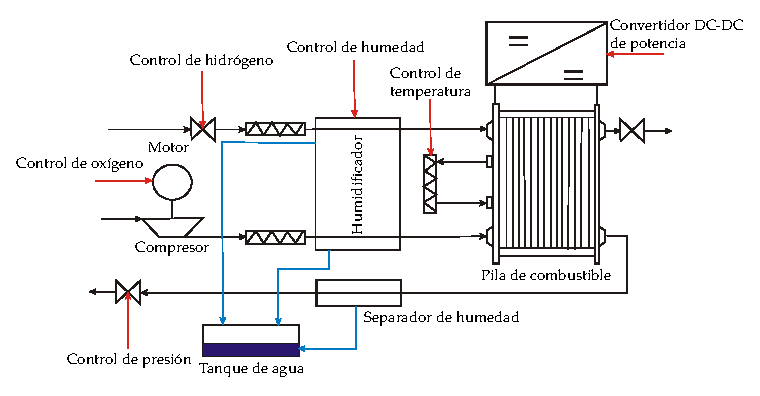
\includegraphics[width=11cm]{gfx/sistema_de_pila_de_combustible.eps}
 \caption{Sistema de celdas de combustible tipo PEM}
 \label{fig:sistema_pila}
\end{figure}

Aunque esos componentes auxiliares pueden variar, se explican los que se presentan en la mayoría de los sistemas:

\begin{itemize}
 \item \textbf{Suministro de combustible}: Se encarga de proporcionar el combustible con la pureza y la presión apropiadas hacia
 el colector. Para el caso de las PEMFC es necesario que la pureza sea muy alta para no dañar los electrodos.
 \item \textbf{Suministro de aire}: Este módulo involucra el uso de compresores o tanques de aire comprimido junto con filtros.
 \item \textbf{Gestión térmica}: Es necesaria una temperatura precisa para que la pila opere adecuadamente.
 \item \textbf{Humidificación}: El agua no solo participa de la operación de las pilas como producto de las reacción producidas sino que también
 es preciso que los gases estén compuestos por una determinada cantidad de vapor de agua. Por otra parte el agua producida por la pila debe ser
 evacuada y además constituye un indicador de la energía eléctrica producida por el sistema.
 \item \textbf{Acondicionamiento de potencia}: La energía eléctrica entregada se realiza mediante una etapa que se encargue de adecuar los niveles
 eléctricos. Ésta etapa es la que adapta el sistema de la pila a la red se conecte. Para el caso del SGH del proyecto,
 proporciona la interfaz entre el módulo de celdas de combustible y el bus de continua que interconecta todo el sistema.
\end{itemize}

\section{Consideraciones energéticas}
La energía liberada durante la actividad de la pila se estudia mediante la energía libre de Gibbs. En (\ref{eq:reaccion_basica}),
el término $\Delta \overline{g}_f$ hace referencia a la diferencia en el cambio de la energía de Gibbs entre reactivos y productos por mol
consumido. Partiendo de este concepto pueden encontrarse una serie de relaciones de gran utilidad. La carga que fluye en el circuito externo
por mol de hidrógeno consumido según ( \ref{eq:reaccion_hidrogeno}) es $ -2Ne = -2F $, siendo $N$ el número de Avogadro, $e$ la carga de
un solo electrón y $F$ la constante de Faraday. Si se asume que toda la energía liberada lo hace como energía eléctrica, es decir el proceso
es reversible, se tiene:
$$ \Delta \overline{g}_f = carga \times tensi \acute{o}n = -2FE $$
Es decir,
\begin{equation}
 E=-\frac{\Delta \overline{g}_f}{2F}
\end{equation}
Donde $E$ representa la fuerza electromotriz de la celda. Por ejemplo a $80$\textcelsius, $E=1.17V$, basado en
cálculos de la diferencia de energía liberada para la reacción estudiada.

Esta magnitud será utilizada más adelante al momento de definir los modelos de tensión de la pila de celdas de combustible. Además, puede ser 
utilizada para hallar la eficiencia de la pila en una dada condición de operación, comparándose la tensión real entregada por la pila y la
fuerza electromotriz. Para que éste calculo sea preciso se debe incluir la proporción de reactivos que efectivamente se consume en la reacción,
\begin{equation}
 \eta=\mu_f\frac{U_c}{E}\times100\%
\end{equation}
Donde $U_c$ es la tensión real entregada por la celda, y $\mu_f$ es el coeficiente de utilización del combustible.

La tensión $E$ o fuerza electromotriz es también llamada de \emph{ tensión reversible de circuito abierto} ya que representaría la tensión que la pila
ofrecería teóricamente si no entregase corriente, aunque en la práctica es levemente menor.

A medida que la corriente demandada a la celda aumenta, la tensión disminuye, a su vez también lo hace la eficiencia. Son varios los motivos
por los cuales la celda se comporta así y esto será estudiado en el cap. \ref{ch:modelo}. En general existen tres regiones
diferenciadas, la fig. \ref{fig:caracteristica_electrica} muestra estas regiones.

\begin{figure}[H]
 \centering
 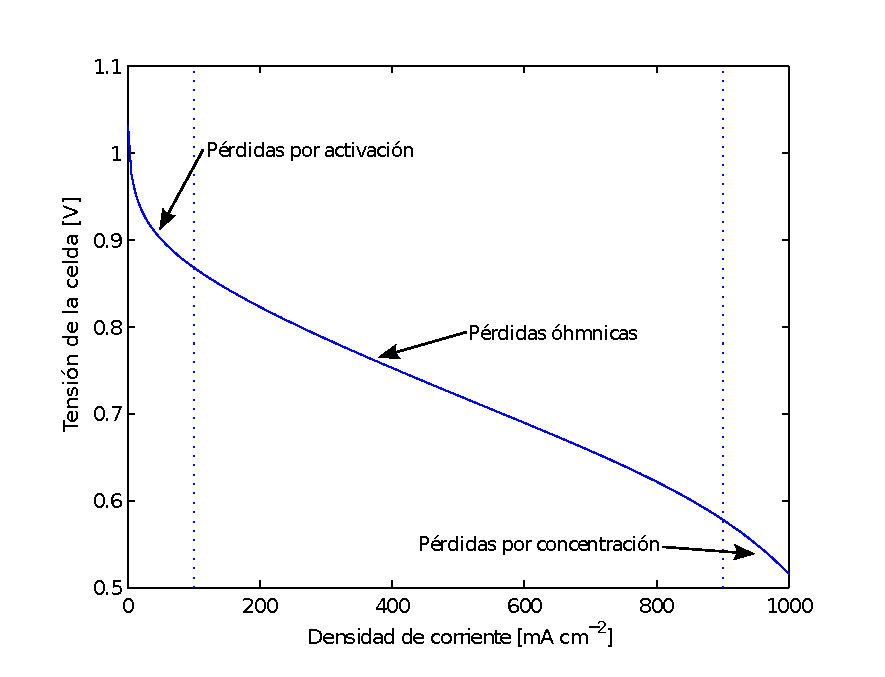
\includegraphics[width=10cm]{gfx/cacteristica_electrica_inf.eps}
 \caption{Característica típica de tensión-densidad de corriente.}
 \label{fig:caracteristica_electrica}
\end{figure}



\section{Comentarios}
Las celdas de combustible han sido presentadas y se han comentado varias de su principales cualidades. Entre ellas se han encontrado algunas
ventajas y otros inconvenientes.
El panorama brindado en éste capítulo ha servido como soporte teórico al trabajo desarrollado para la construcción del emulador de celdas de combustible
y permitirá proseguir al siguiente capítulo que se centra en las características eléctricas en los modelos adoptados para el diseño.
\end{comment}
